In Hops for reasons that I have outlines in previous chapters we
persist all the metadata in our persistent storage solution. MySQL
Cluster is a relational distributed database, so data is stored into
tables with very specific properties. Since version 7.3.1, MySQL
Cluster supports foreign key constraints. Foreign keys is a powerful
feature of relational databases that guarantee some kind of
consistency between two tables. One important aspect of foreign keys
is that they map relationships of the ``real-world'' into
relationships in the database.

The database schema of Hops consists of 95 tables, 64 out of them are
used by Hops-YARN. The information they store span from incoming RPCs
to scheduler state and nodes' statuses. We make heavy use of foreign
key constraints, mainly the \texttt{ON DELETE} referential action, to
ensure integrity when a row from a parent table is deleted. Although
the database schema of Hops-YARN is too big to fit in
a single page, Figure \ref{fig:impl_fk_yarn_schema}, the number of
foreign key relationships -- they are illustrated with a solid line --
is clear.

*** Say why this is bad in terms of performance. Subsection for each
parent table and how I dealt with it

\begin{figure}
\centering
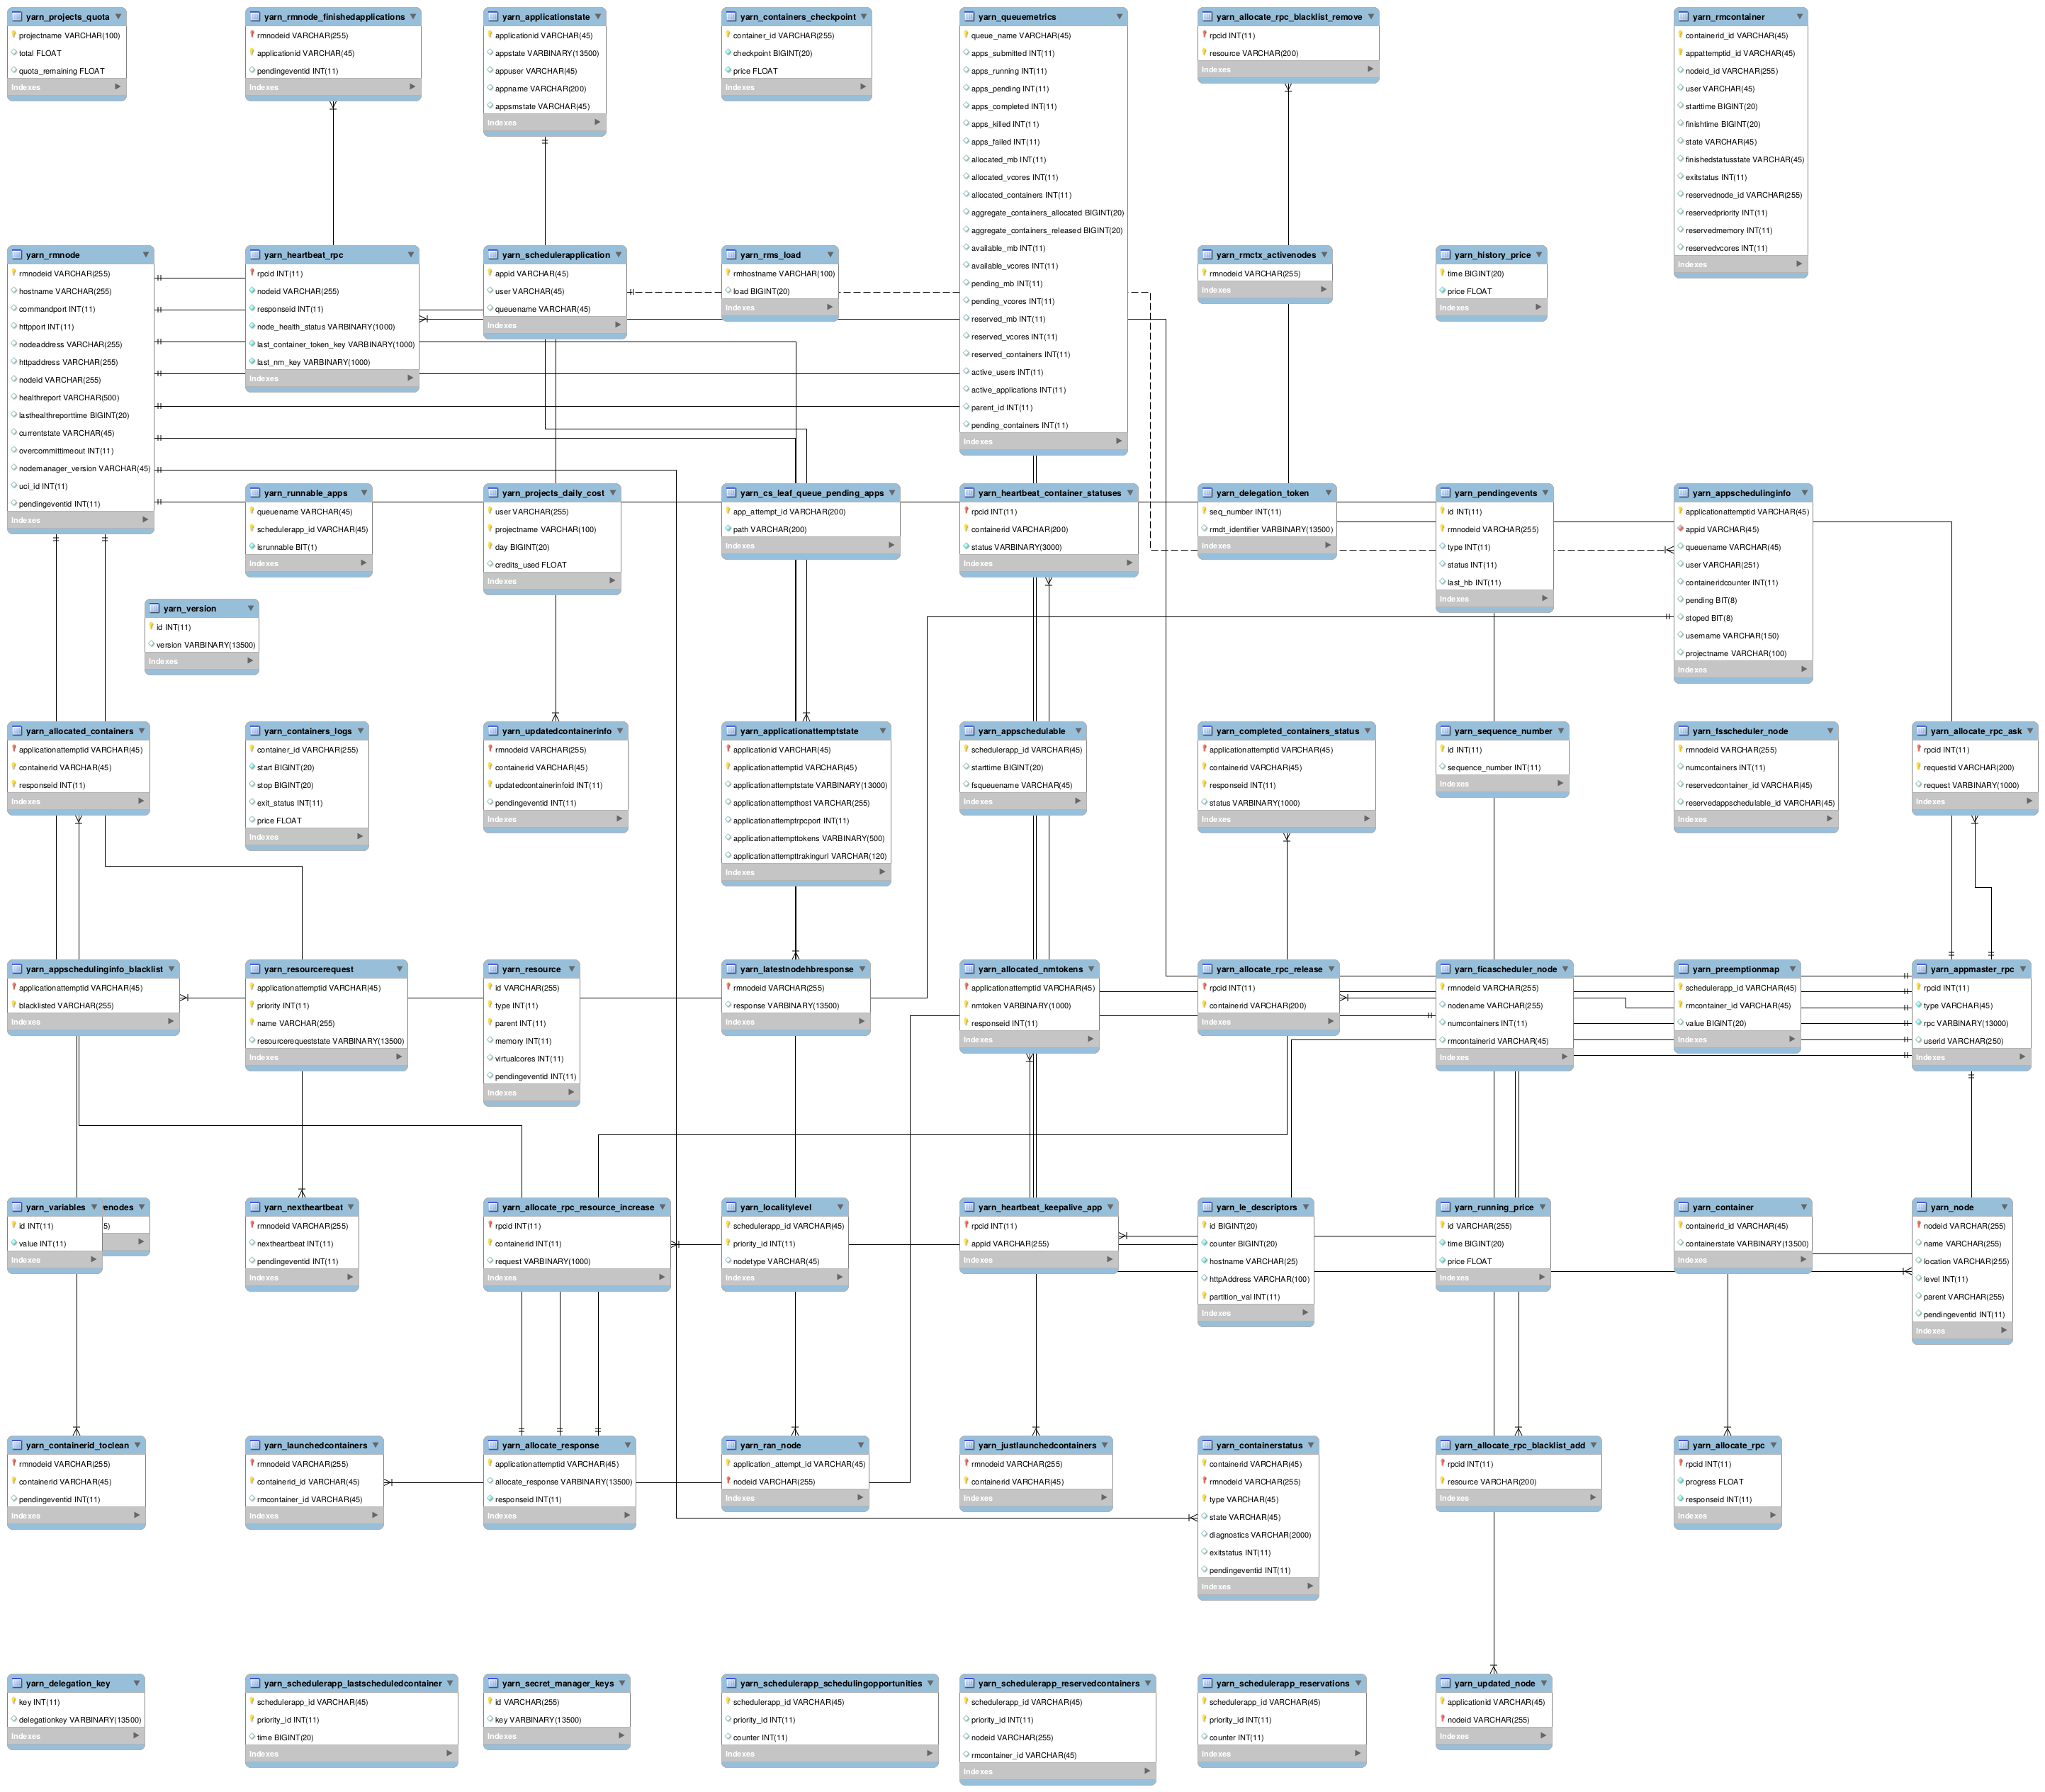
\includegraphics[scale=0.2, angle=90]{resources/images/Implementation/hops_yarn_ndb_schema_full.png}
\label{fig:impl_fk_yarn_schema}
\caption{Hops-YARN database schema}
\end{figure}